\Chapter{Introduzione}
\Section{Contesto}

La segmentazione di strutture anatomiche in immagini mediche 3D rappresenta un task importante nell’ambito clinico e diagnostico. In particolare la segmentazione del seno da immagini MRI (Magnetic Resonance Imaging) 3D è un task complesso, ma essenziale per applicazioni come la pianificazione di interventi chirugici o l’analisi di anomalie tessutali.

In passato, la segmentazione del seno in immagini MRI 3D veniva effettuata principalmente con \textbf{metodi classici}, spesso semi-automatici o manuali, basati su:

\begin{itemize}
	\item \hlight{Approcci a soglia} (thresholding) e \hlight{region-growing}, che sfruttavano differenze di intensità tra tessuti ma richiedevano regolazioni manuali e fallivano in presenza di rumore o basso contrasto.
	\item \hlight{Deformable models} (es.: Active Contours) e \hlight{algoritmi a clustering} (es.: k-means), sensibili all’inizializzazione e poco robusti alla variabilità anatomica.
	\item Metodi \hlight{atlas-based}, che allineavano immagini a template pre-annotati, limitati però dalla diversità inter-paziente.
\end{itemize}

Con l’avvento del \textbf{deep learning}, in particolar modo delle \textbf{reti convoluzionali} e di architetture come \hlight{U-Net 3D} \cite{chen2021transunet}, la segmentazione del seno ha raggiunto livelli di accuratezza più alti rispetto al passato. 




\Section{Attività di Tirocinio e obiettivi}

L’attività si è inserita nel contesto di un progetto di ricerca mirato allo sviluppo e alla valutazione di modelli di segmentazione automatica per immagini in MRI del seno, con l’obiettivo di migliorare la diagnosi precoce e la pianificazione terapeutica.

L’obiettivo principale del tirocinio è stato quello di sperimentare e ottimizzare pipeline basate su \textbf{deep learning} per la segmentazione semantica tridimensionale, utilizzando framework open-source moderni come \textbf{MONAI} (Medical Open Network for AI) \cite{cardoso2022monai} e \textbf{PyTorch}.

Le principali attività svolte durante il tirocinio sono state:
\begin{itemize}
    \item \textbf{Pre-processing} dei dati in formato DICOM, con conversione in formato leggibile da MONAI e normalizzazione delle immagini.
    \item Composizione e validazione di un dataset bilanciato, con partizionamento in training, validation e test set.
    \item Studio e implementazione di modelli di segmentazione basati su architetture tra cui \textbf{UNet} e \textbf{AttentionUNet}.
    \item Configurazione degli esperimenti, \textbf{tuning degli iperparametri} e addestramento dei modelli in ambiente GPU.
    \item Valutazione delle prestazioni mediante metriche standard come Dice Score
\end{itemize}

Durante il tirocinio sono state inoltre affrontate e risolte diverse problematiche tecniche legate alla gestione dei metadati DICOM, alla compatibilità tra i formati di input, e alla gestione efficiente della memoria in fase di training. L'intero lavoro è stato documentato e riproducibile mediante script \textbf{Python} e configurazioni \textbf{YAML} modulari.


	
\Section{Strumenti Utilizzati}
Durante il tirocinio sono stati impiegati diversi strumenti software e librerie  fondamentali per la gestione, il pre-processing e l'elaborazione di immagini medicali, nonché per lo sviluppo e il training di modelli di deep learning.
\begin{itemize}
	\item  Il linguaggio principale di lavoro è stato \textbf{Python}, scelto per la sua flessibilità e per l'ampio ecosistema di librerie scientifiche.
	\item Per la manipolazione delle immagini DICOM è stata utilizzata la libreria \textbf{MONAI} (Medical Open Network for AI), un framework open-source basato su PyTorch e progettato specificamente per applicazioni di imaging medicale. MONAI ha permesso di gestire agevolmente il caricamento dei dati, le trasformazioni e la normalizzazione delle immagini, grazie a un sistema modulare di trasformazioni componibili.
	\item Il framework di deep learning impiegato è stato \textbf{PyTorch}, scelto per la sua semplicità d'uso, il supporto attivo della community e le sue prestazioni elevate, specialmente in combinazione con l'accelerazione GPU fornita da CUDA.
	\item Lo sviluppo del codice è stato realizzato su una macchina Linux, con accesso remoto e con l'ausilio dell'editor \textbf{Visual Studio Code}.
\end{itemize}


\Subsection{Connessione in SSH e GPU}

Durante il tirocinio, ho avuto accesso alla potenza di calcolo delle \textbf{GPU universitarie}, dedicate a progetti di ricerca in deep learning. Per sfruttare queste risorse, ho utilizzato il protocollo \textbf{SSH} (Secure Shell) \ref{fig:gpu_info} per connettermi in remoto ai server e gestire l’esecuzione dei miei esperimenti.

Il sistema era dotato di 4 GPU NVIDIA (modello Tesla V100 o A100, a seconda della disponibilità), condivise tra diversi utenti del dipartimento. Per evitare conflitti nell’allocazione delle risorse, è stato necessario prenotare in anticipo le GPU tramite un sistema di schedulazione interno, basato su code di priorità.

Nel dettaglio, il nodo su cui ho lavorato disponeva delle seguenti GPU:
\begin{itemize}
\item \textbf{3x NVIDIA Tesla V100-PCIE-16GB}, GPU ad alte prestazioni con 16 GB di memoria, molto diffuse in ambito scientifico per il training di deep neural networks.
\item \textbf{1x NVIDIA A100 80GB PCIe}, una delle GPU più potenti attualmente disponibili per il calcolo scientifico, con ben 80 GB di memoria dedicata. 
\end{itemize}

Le informazioni mostrate da \texttt{nvidia-smi} includevano anche temperatura, consumo energetico, utilizzo della memoria e livello di attività di ciascuna GPU. 

Questa infrastruttura ha permesso di testare i miei modelli su dataset di grandi dimensioni con tempi di addestramento molto più rapidi rispetto all’uso di una macchina locale.

\begin{figure}[H] 
  	\centering 
 	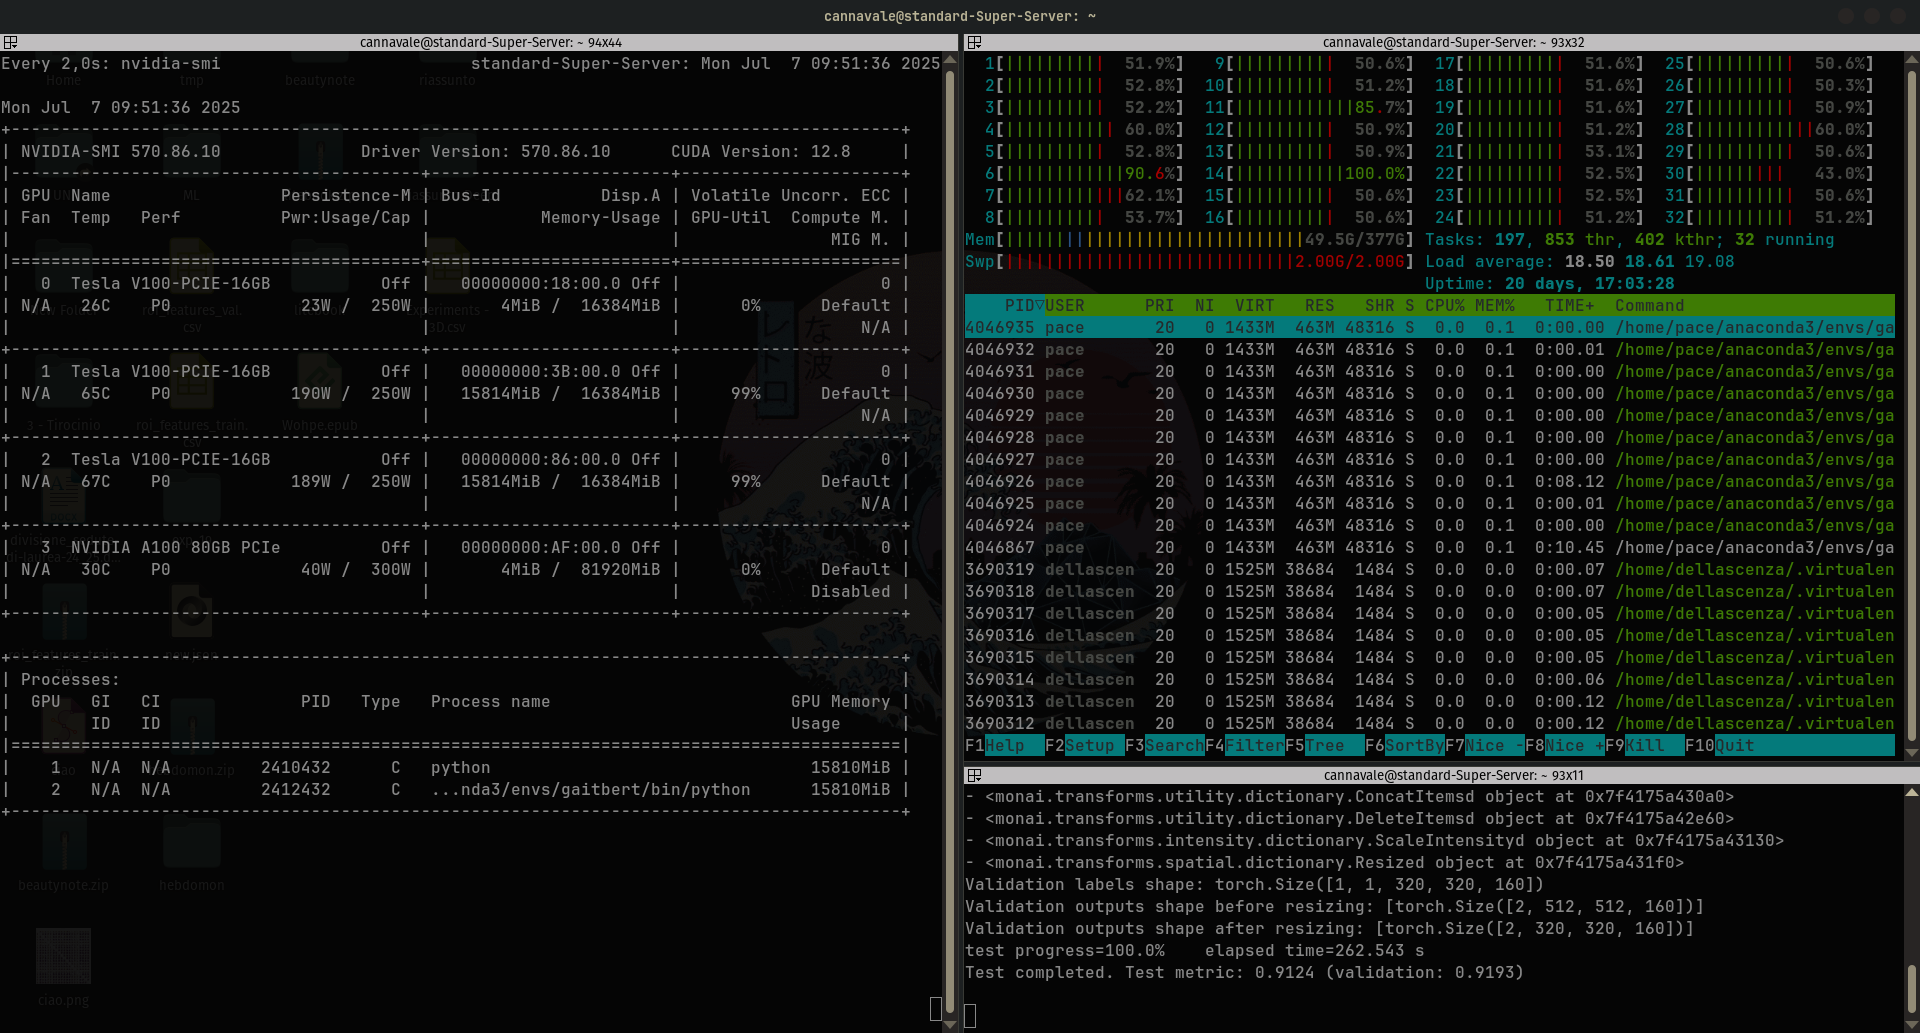
\includegraphics[width=\textwidth]{images/2025-07-07-09-52-55.png} 
	\label{fig:gpu_info}
	\caption{Esempio di output del comando \texttt{nvidia-smi} per monitorare le GPU disponibili.}
 \end{figure} 